% !TEX encoding = UTF-8 Unicode
%!TEX root = thesis.tex
% !TEX spellcheck = en-US
%%=========================================



\chapter{Results}\label{chap:results}




The results in this research project are mainly gathered from the final test session, which was held after the last development stage, thus the results reflect the state of the application at the end of the research. 

The test sessions had two separate qualitative data gathering strategies: 

A multiple choice knowledge test taken by the test participants before and after the session,  this was meant to demonstrate learning value in short term time frame. Such a simple short term test could support the claim that the artifact can be used as an educational tool. The test is attached as \autoref{chap:knowtest}.
The second strategy was a combined SUS questionnaire with general questions about the application. This questionnaire can be found as \autoref{chap:questionnaire}.
The knowledge test was taken by the medical students in test sessions, while the questionnaire was answered by six participants, of which four were medical students.

% though further research is needed.

\section{Educational value}





\section{Usability}

The usability results are based on the second test session where a questionnaire, including a SUS section, was uses in addition to unstructured feedback from the test participants. The results from these methods will be presented in this section. 

\subsection{System usability scale questionnaire}
 
The SUS questionnaire was taken by six participants, five answering based on the HoloLens 2 experience and one based on using the Android application. The mean score from the HoloLens 2 is $79.0 \pm 10.4$, while the result from the single Android test was 75. This means that the application on HoloLens 2 sits high in the good rating almost reaching excellent, while the Android app is near the middle of the good rating. \autoref{fig:susresults} show the results of the SUS questionnaire charted with the red line representing the 68 \textit{average} score.

\begin{figure}
    \centering
    \textbf{SUS results}\par\medskip
    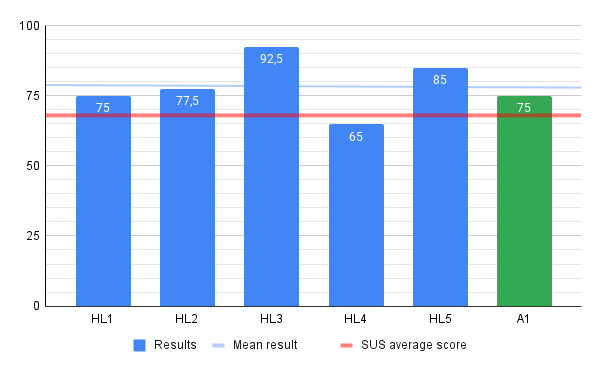
\includegraphics[width=0.75\textwidth]{fig/susbarchart}
    \caption{The blue results are from HoloLens 2, while the green is from Android.}
    \label{fig:susresults}
\end{figure}


\subsection{Research specific questionnaire}
The questionnaire included a section with research specific questions written by the researcher with the aim to gather data relating to the research questions of the project. The question were, just as in SUS, based on the \textit{Likert scale}, with answer alternatives ranging from 1 - 5 indicating how much in agreement the user is with the statement. The section was answered by six participants, and it was platform independent.
% Please add the following required packages to your document preamble:
% \usepackage[table,xcdraw]{xcolor}
% If you use beamer only pass "xcolor=table" option, i.e. \documentclass[xcolor=table]{beamer}
% \usepackage[normalem]{ulem}
% \useunder{\uline}{\ul}{}
\begin{table}[h]
\centering
\textbf{Results from research questionnaire}\par\medskip
\begin{tabular}{l|ccccc}
\hline
                                                                                                                                                          & \begin{tabular}[c]{@{}c@{}}Strongly\\ disagree\end{tabular} & Disagree                                                  & Neutral                                                   & Agree                                                     & \begin{tabular}[c]{@{}c@{}}Strongly\\ agree\end{tabular}  \\ \hline
\begin{tabular}[c]{@{}l@{}}I got new insight about neuroanatomy \\ while using the system.\end{tabular}                                                   & \textbf{}                                                   & \textbf{}                                                 & \textbf{}                                                 & \cellcolor[HTML]{6434FC}{\color[HTML]{EFEFEF} \textbf{4}} & \cellcolor[HTML]{9698ED}{\color[HTML]{EFEFEF} \textbf{2}} \\
\rowcolor[HTML]{EFEFEF} 
\begin{tabular}[c]{@{}l@{}}I got new insight about neuroanatomy \\ while seeing and manipulating the \\ brain and its structures in 3D.\end{tabular}      & \textbf{}                                                   & \textbf{}                                                 & \textbf{}                                                 & \cellcolor[HTML]{9698ED}{\color[HTML]{EFEFEF} \textbf{2}} & \cellcolor[HTML]{6434FC}{\color[HTML]{EFEFEF} \textbf{4}} \\
\begin{tabular}[c]{@{}l@{}}I got new insight about neuroanatomy \\ while dissecting the brain.\end{tabular}                                               & \textbf{}                                                   & \textbf{}                                                 & \cellcolor[HTML]{CBCEFB}{\color[HTML]{EFEFEF} \textbf{1}} & \cellcolor[HTML]{6200C9}{\color[HTML]{EFEFEF} \textbf{5}} & \textbf{}                                                 \\
\rowcolor[HTML]{EFEFEF} 
\cellcolor[HTML]{EFEFEF}\begin{tabular}[c]{@{}l@{}}I felt like I was collaborating with another \\ person when using the system with others.\end{tabular} & \cellcolor[HTML]{CBCEFB}{\color[HTML]{EFEFEF} \textbf{1}}                           & \cellcolor[HTML]{CBCEFB}{\color[HTML]{EFEFEF} \textbf{1}}                         & \cellcolor[HTML]{6665CD}{\color[HTML]{EFEFEF} \textbf{3}} & \cellcolor[HTML]{CBCEFB}{\color[HTML]{EFEFEF} \textbf{1}}                         & \cellcolor[HTML]{EFEFEF}\textbf{}                         \\
\begin{tabular}[c]{@{}l@{}}I was aware of what the other person did \\ and had focus on when using the system.\end{tabular}                               & \textbf{}                                                   & \cellcolor[HTML]{9698ED}{\color[HTML]{EFEFEF} \textbf{2}} & \cellcolor[HTML]{6665CD}{\color[HTML]{EFEFEF} \textbf{3}} & \cellcolor[HTML]{CBCEFB}{\color[HTML]{EFEFEF} \textbf{1}} & \textbf{}                                                 \\
\rowcolor[HTML]{EFEFEF} 
\begin{tabular}[c]{@{}l@{}}The system would be useful for remote \\ teaching of neuroanatomy.\end{tabular}                                                & \textbf{}                                                   & \textbf{}                                                 & \cellcolor[HTML]{CBCEFB}{\color[HTML]{EFEFEF} \textbf{1}} & \cellcolor[HTML]{9698ED}{\color[HTML]{EFEFEF} \textbf{2}} & \cellcolor[HTML]{6665CD}{\color[HTML]{EFEFEF} \textbf{3}} \\ \hline
\end{tabular}
\caption{The results form the research specific questions, the number and color values represent the magnitude of answers with the corresponding alternative.}
\end{table}

\subsection{IPEAR AR and peer learning questionnaire}
This section was included as part of other research at the NTNU VRLab

\begin{table}[]
\centering
\begin{tabular}{l|ccccc}
\hline
                                                                                                                                             & \begin{tabular}[c]{@{}c@{}}Strongly\\ disagree\end{tabular} & Disagree                                                  & Neutral                                                   & Agree                                                     & \begin{tabular}[c]{@{}c@{}}Strongly\\ agree\end{tabular}  \\ \hline
\begin{tabular}[c]{@{}l@{}}Did you like the approach of peer learning \\ \small{(working with and teaching your classmates)}?\end{tabular}           & \textbf{}                                                   & \textbf{}                                                 & \cellcolor[HTML]{6665CD}{\color[HTML]{EFEFEF} \textbf{3}} &  & \cellcolor[HTML]{6665CD}{\color[HTML]{EFEFEF} \textbf{3}} \\
\rowcolor[HTML]{EFEFEF} 
\begin{tabular}[c]{@{}l@{}}Were you more interested in teaching \\each other  and sharing content with \\your peers and AR tools?\end{tabular} & \textbf{}                                                   & \cellcolor[HTML]{CBCEFB}{\color[HTML]{EFEFEF} \textbf{1}} & \cellcolor[HTML]{CBCEFB}{\color[HTML]{EFEFEF} \textbf{1}} & \cellcolor[HTML]{6434FC}{\color[HTML]{EFEFEF} \textbf{4}} & {\color[HTML]{EFEFEF} \textbf{}}                          \\
\begin{tabular}[c]{@{}l@{}}Did this learning approach make you feel \\ more responsible for your learning?\end{tabular}                      & \textbf{}                                                   & \cellcolor[HTML]{CBCEFB}{\color[HTML]{EFEFEF} \textbf{1}} & \cellcolor[HTML]{6665CD}{\color[HTML]{EFEFEF} \textbf{3}} & \cellcolor[HTML]{CBCEFB}{\color[HTML]{EFEFEF} \textbf{1}} & \cellcolor[HTML]{CBCEFB}{\color[HTML]{EFEFEF} \textbf{1}} \\
\rowcolor[HTML]{EFEFEF} 
\begin{tabular}[c]{@{}l@{}}Do you think it would be useful in other \\ courses or fields of study as well?\end{tabular}                      & {\color[HTML]{EFEFEF} \textbf{}}                            & {\color[HTML]{EFEFEF} \textbf{}}                          & {\color[HTML]{EFEFEF} \textbf{}}                          & \cellcolor[HTML]{9698ED}{\color[HTML]{EFEFEF} \textbf{2}} & \cellcolor[HTML]{6434FC}{\color[HTML]{EFEFEF} \textbf{4}} \\ \hline
\end{tabular}
\end{table}


\subsection{Feedback from participants}

During the test sessions the participants gave feedback on their thoughts of the application, and how to improve the user experience.






%====================================================

% % The result of this project is the preliminary work for my master thesis next semester, thus 

% \section{Nevrolens}\label{nevrolens}
% Nevrolens is the name I've given the application which is the research product of this project. It's a combination of the Norwegian word Nevroanatomi and HoloLens. It is a AR application running on HoloLens 1, HoloLens 2 and Android. 

% The application is focused on delivering a single user experience, with features as cutting planes, scaling, moving brain parts and transparent brain parts. \autoref{fig:nevrolens_holo} show these features running on HoloLens 2, while \autoref{fig:nevrolens_android} show them on Android.
% It is packages and released on GitLab at \url{https://gitlab.stud.idi.ntnu.no/imtel/nevrolens}. 

% \begin{figure}[h]\label{fig:nevrolens_holo}
%     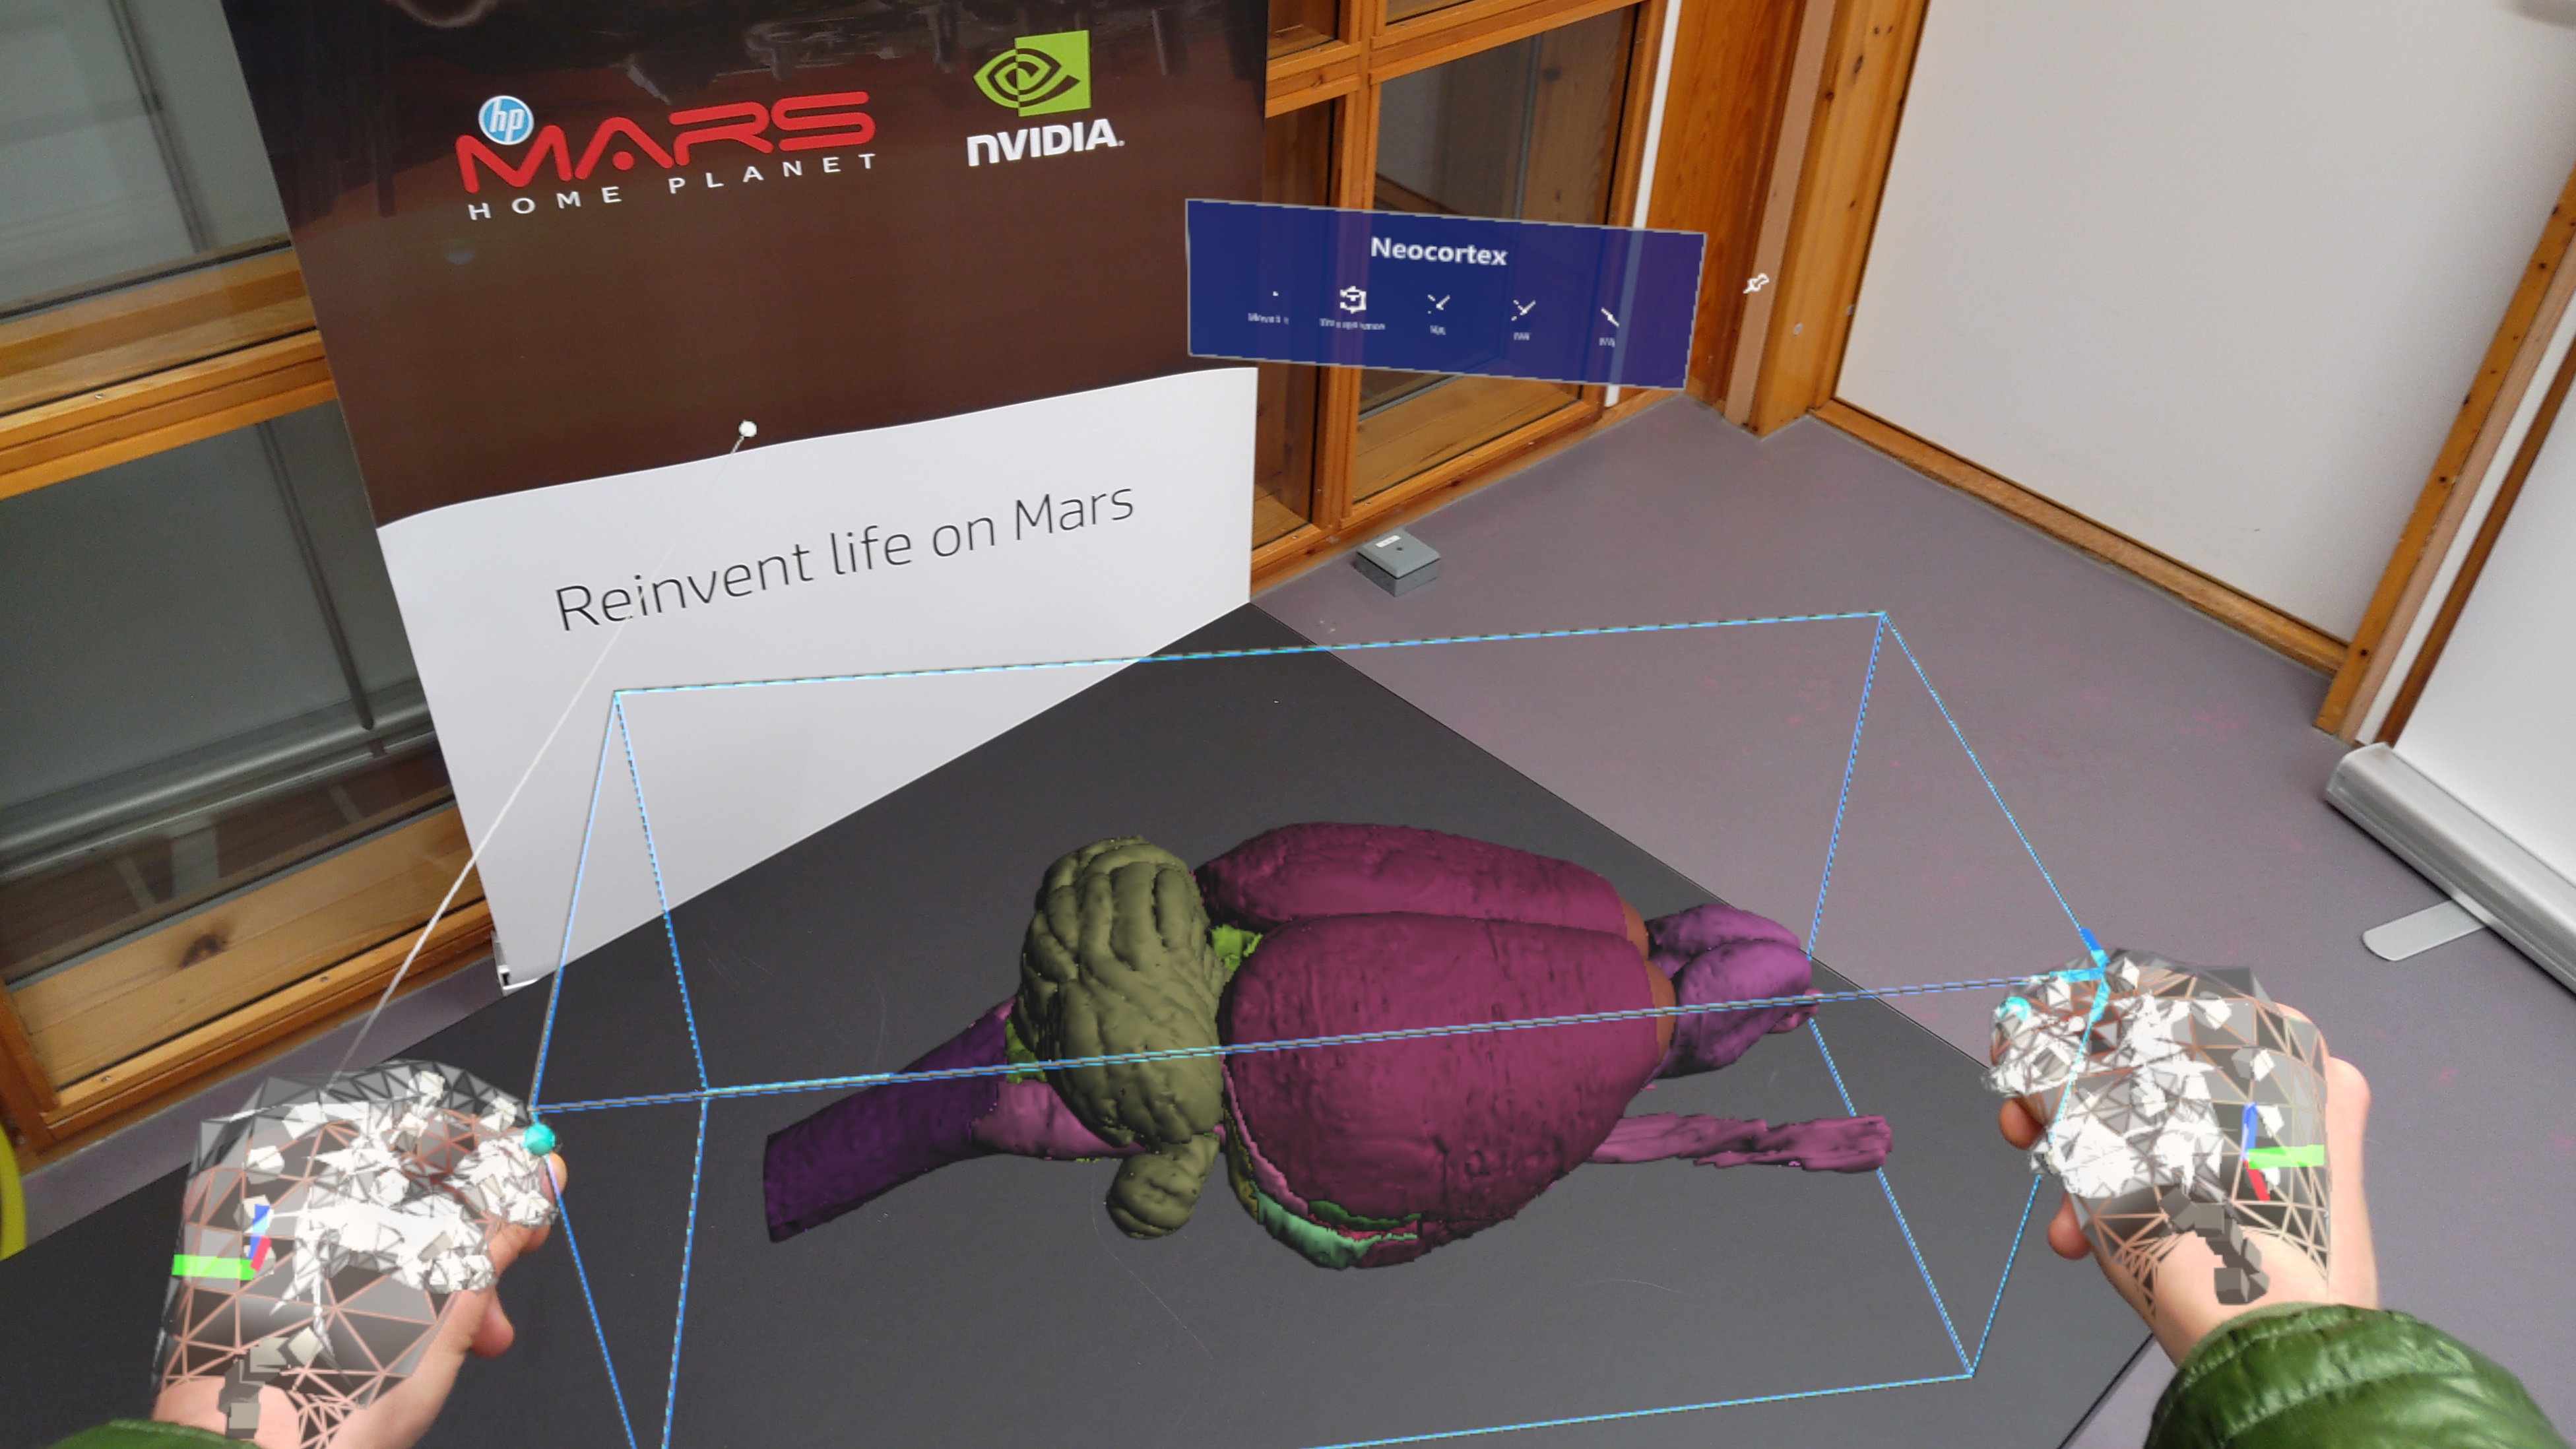
\includegraphics[width=0.5\textwidth]{fig/nevrolens/twohandedzoom.jpg}
%     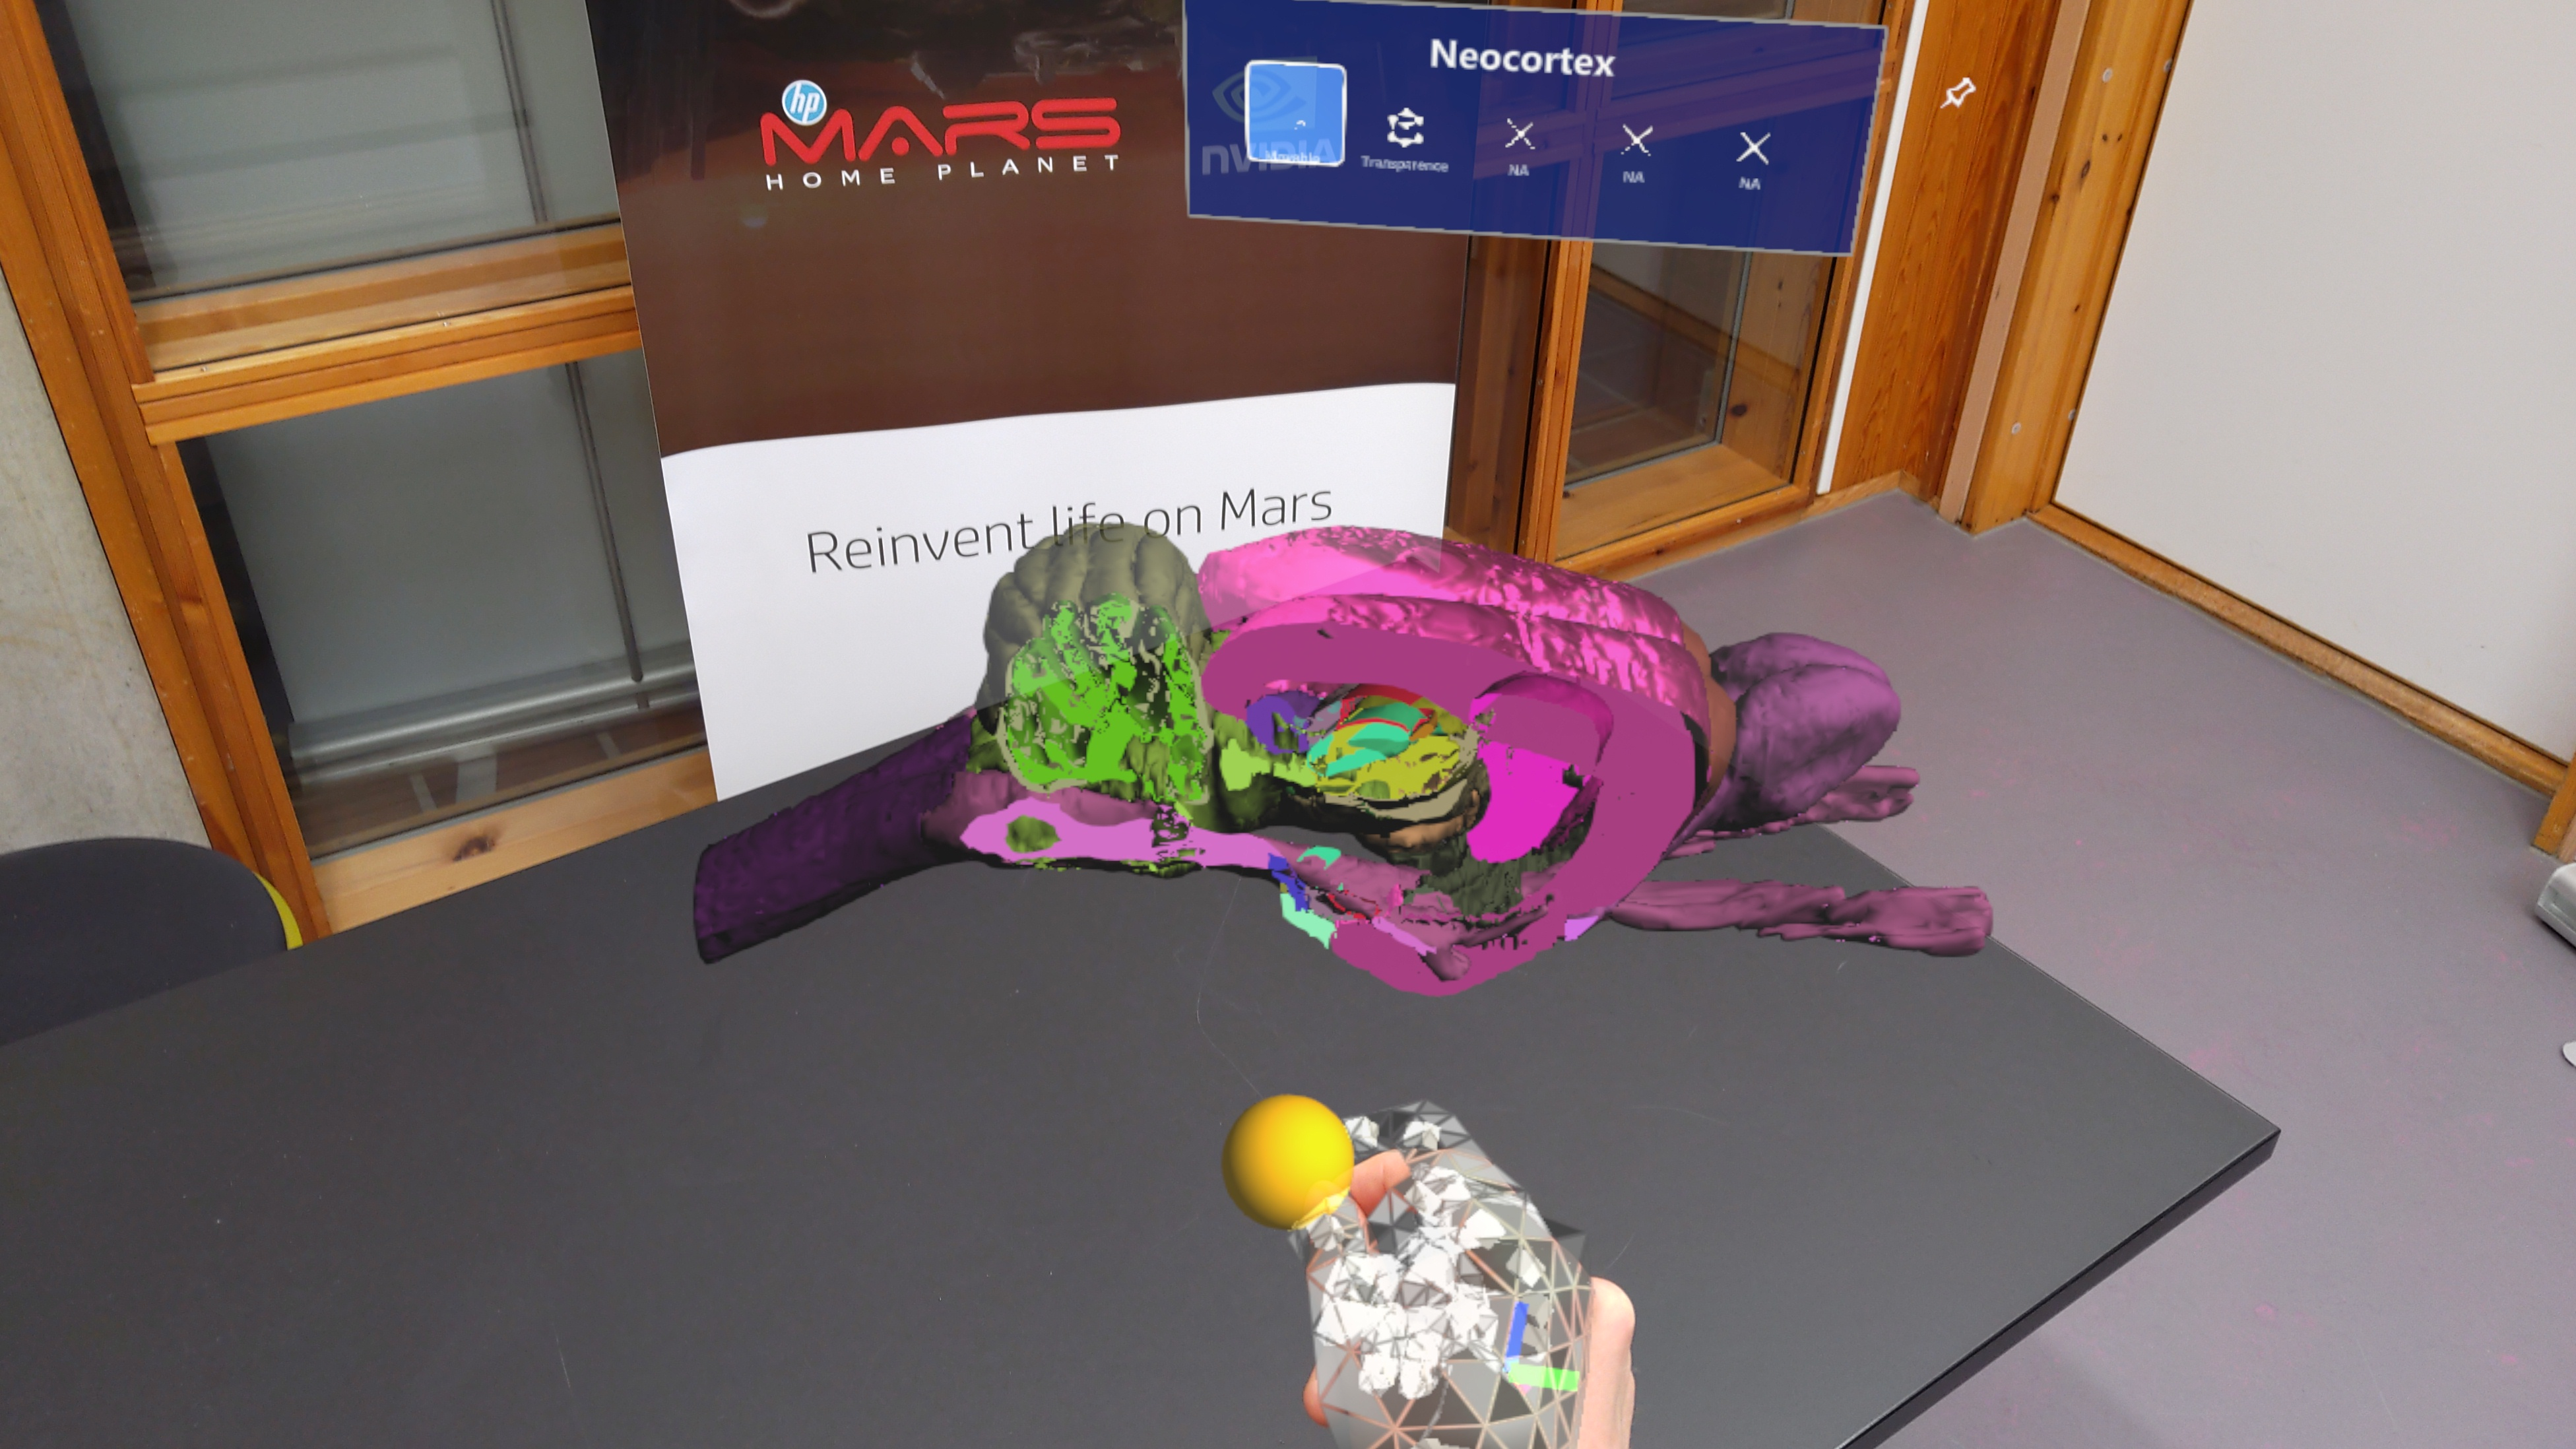
\includegraphics[width=0.5\textwidth]{fig/nevrolens/clipping.jpg}
%     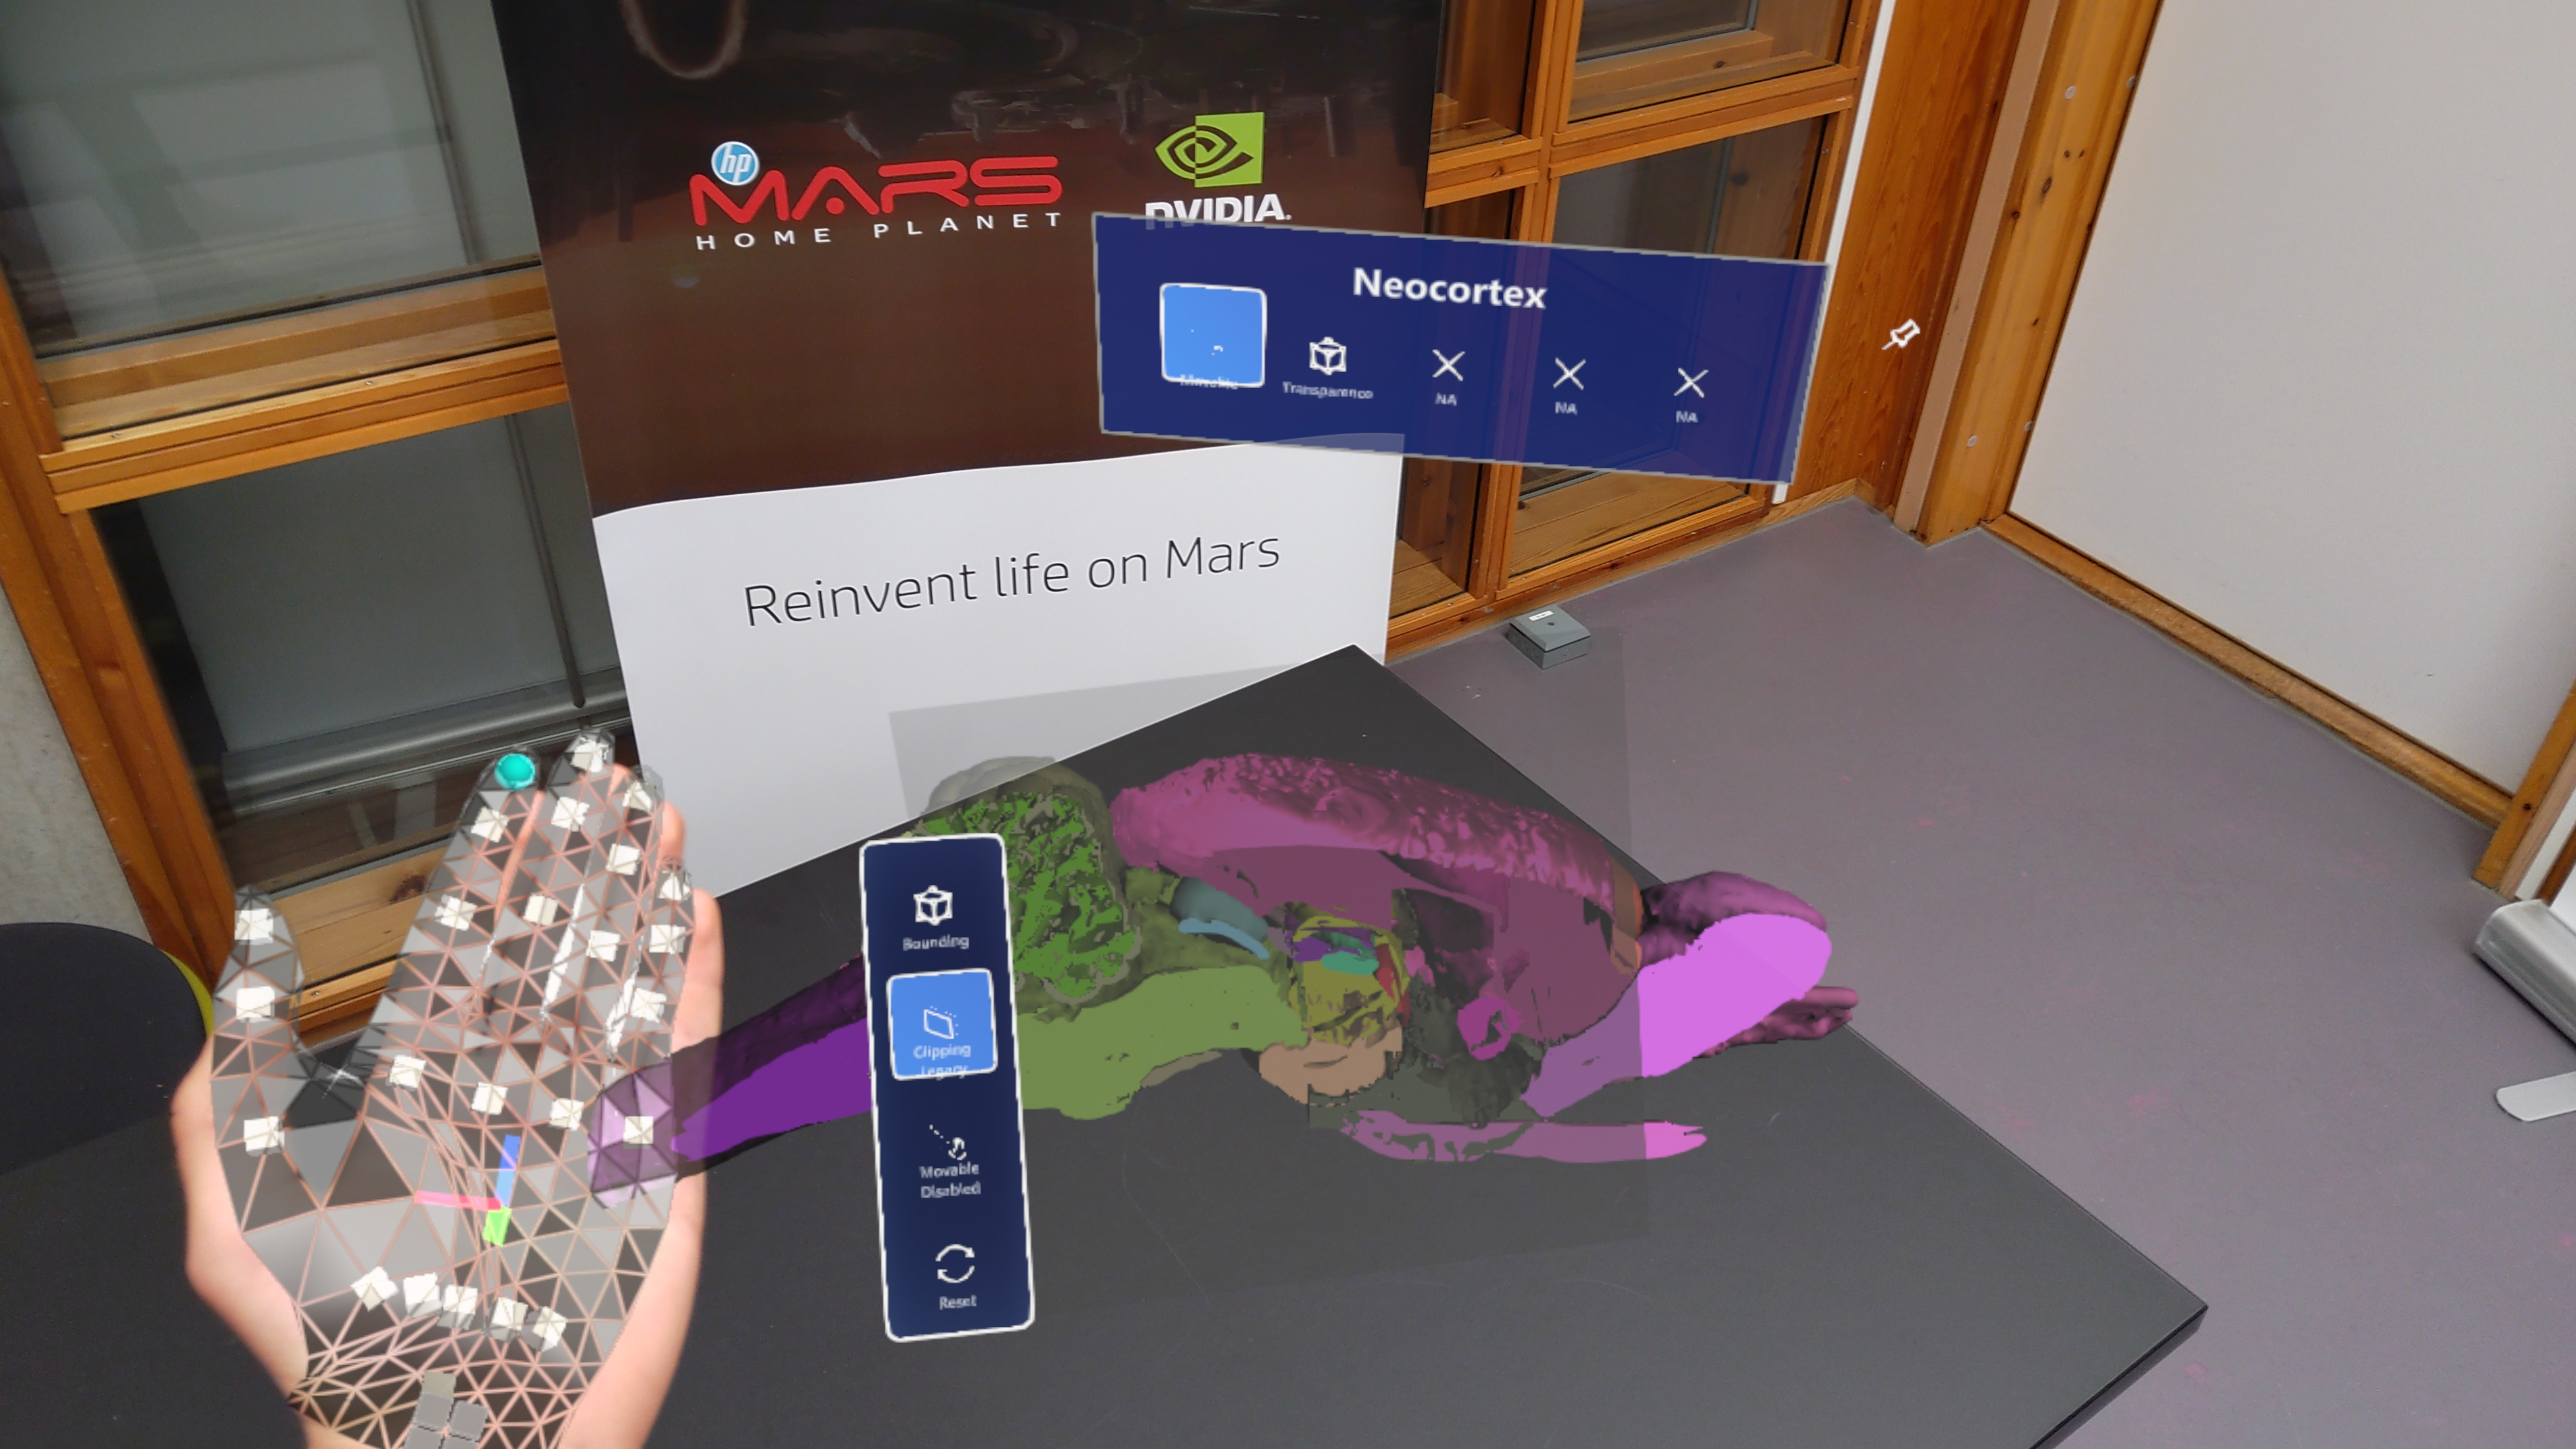
\includegraphics[width=0.5\textwidth]{fig/nevrolens/palmmenu.jpg}
%     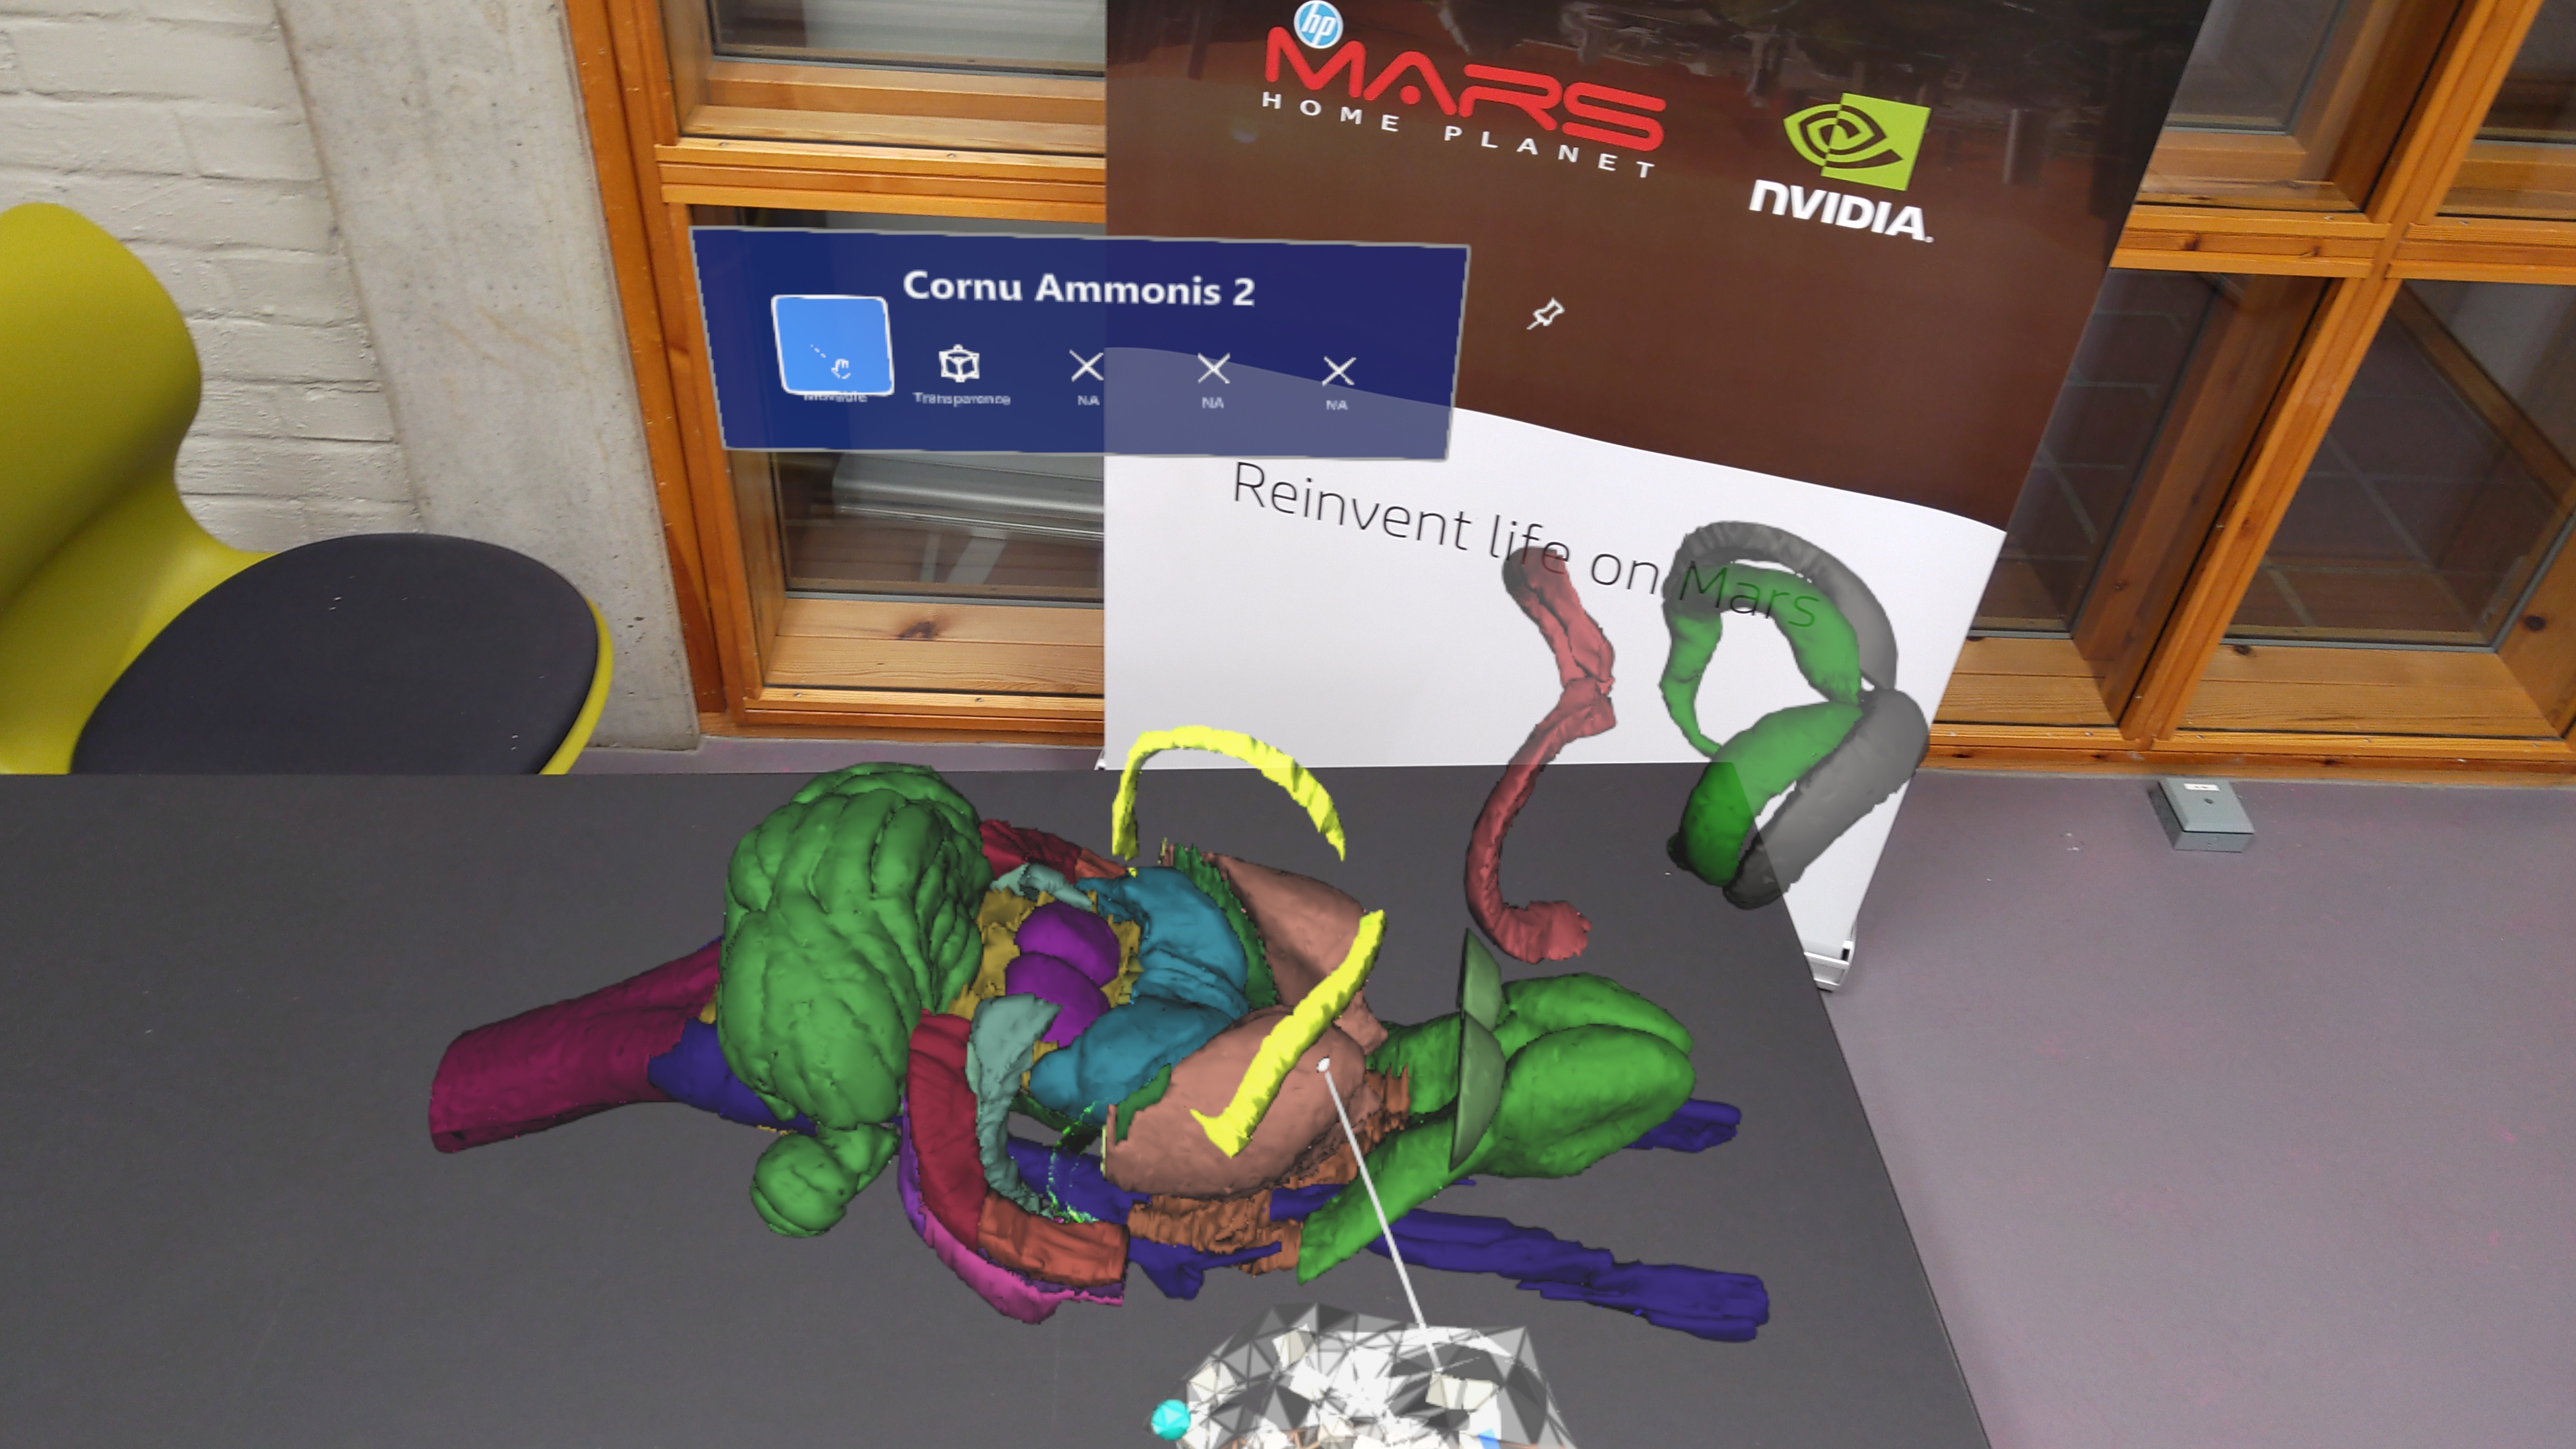
\includegraphics[width=0.5\textwidth]{fig/nevrolens/brainpartsout.jpg}
%     \caption{Nevrolens v0.1.3 on HoloLens 2}
% \end{figure}


% \begin{figure}[h]\label{fig:nevrolens_android}
%     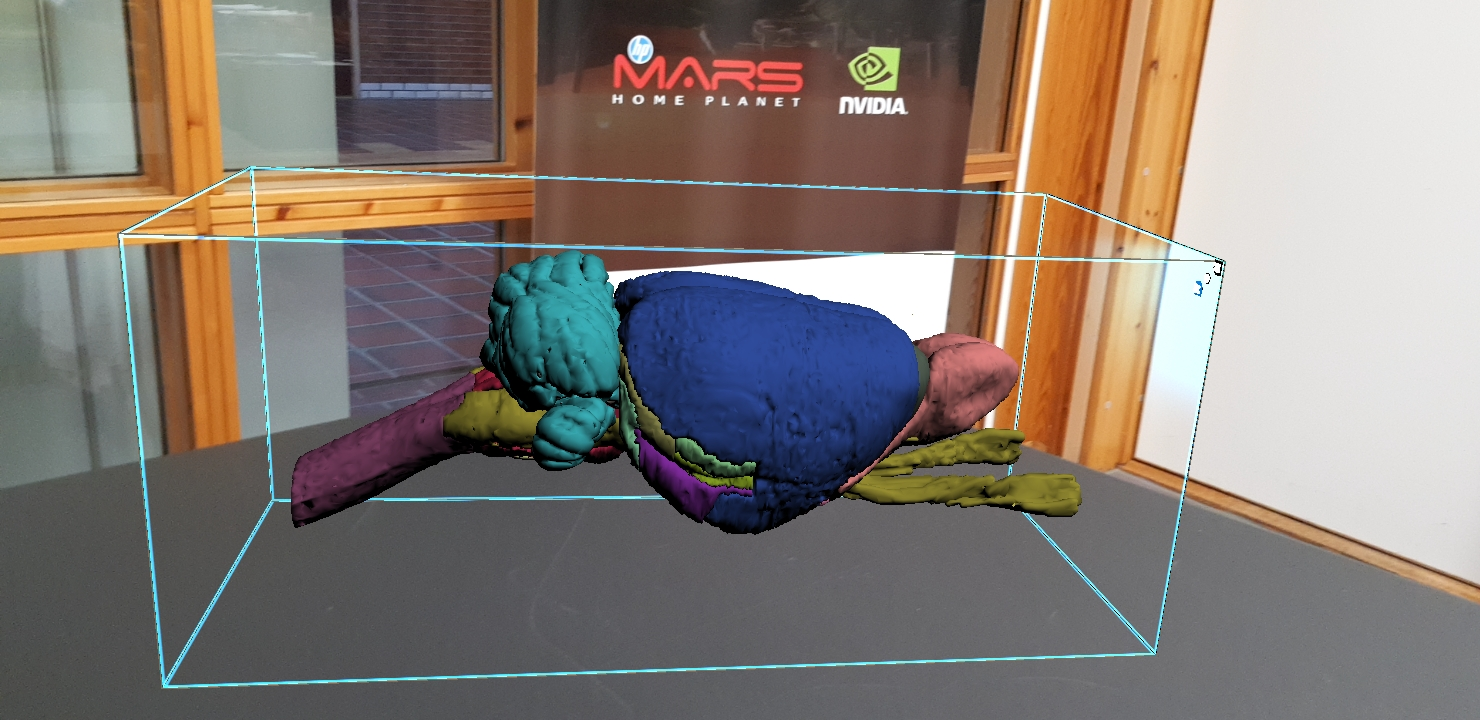
\includegraphics[width=0.5\textwidth]{fig/nevrolens/android_zoom_large.jpg}
%     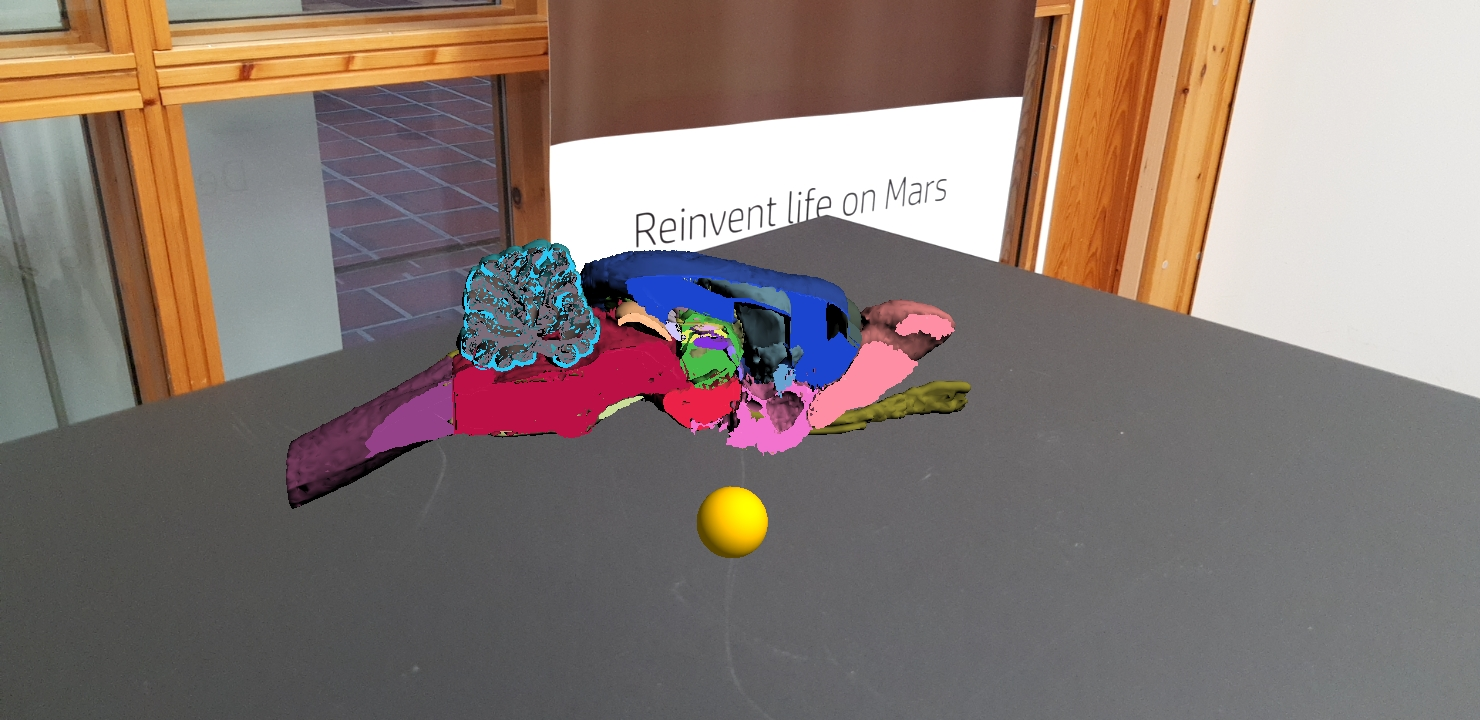
\includegraphics[width=0.5\textwidth]{fig/nevrolens/android_clipping.jpg}
%     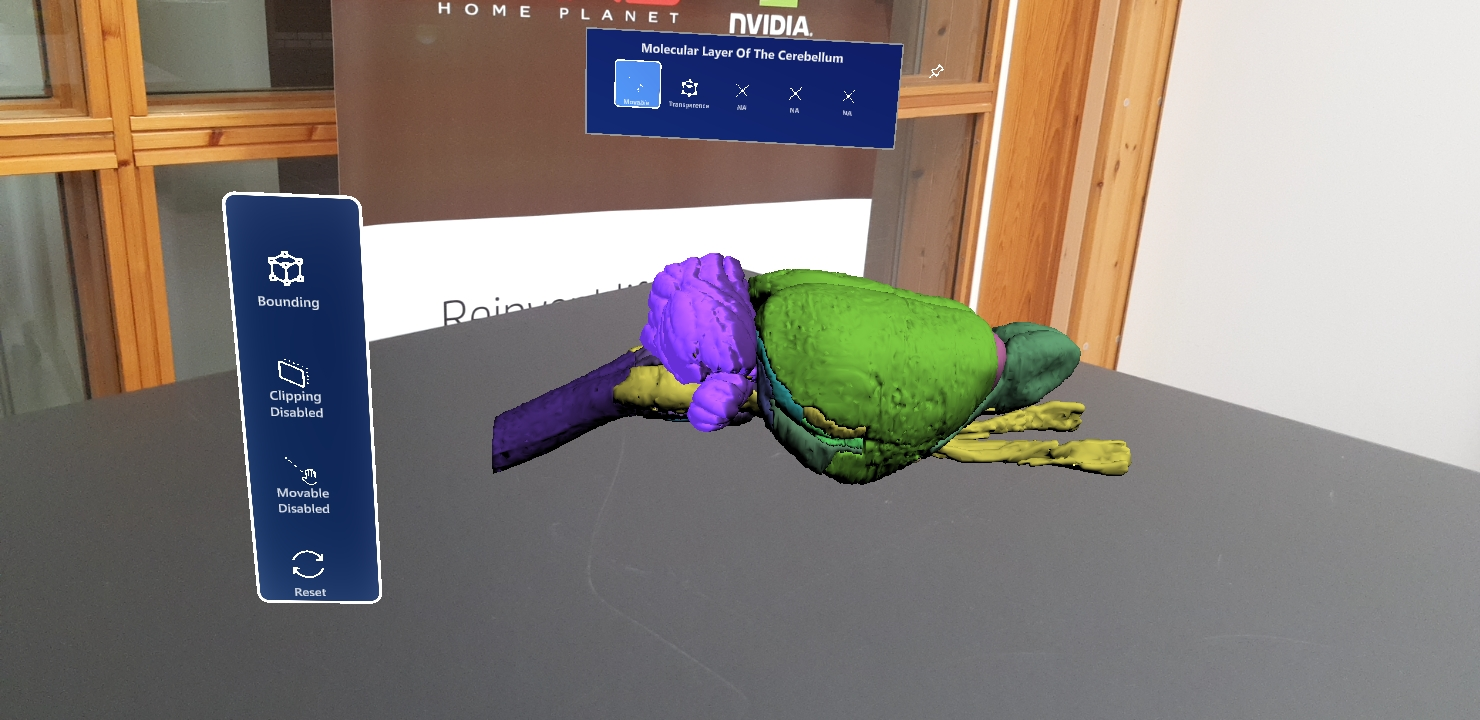
\includegraphics[width=0.5\textwidth]{fig/nevrolens/android_palmmenu.jpg}
%     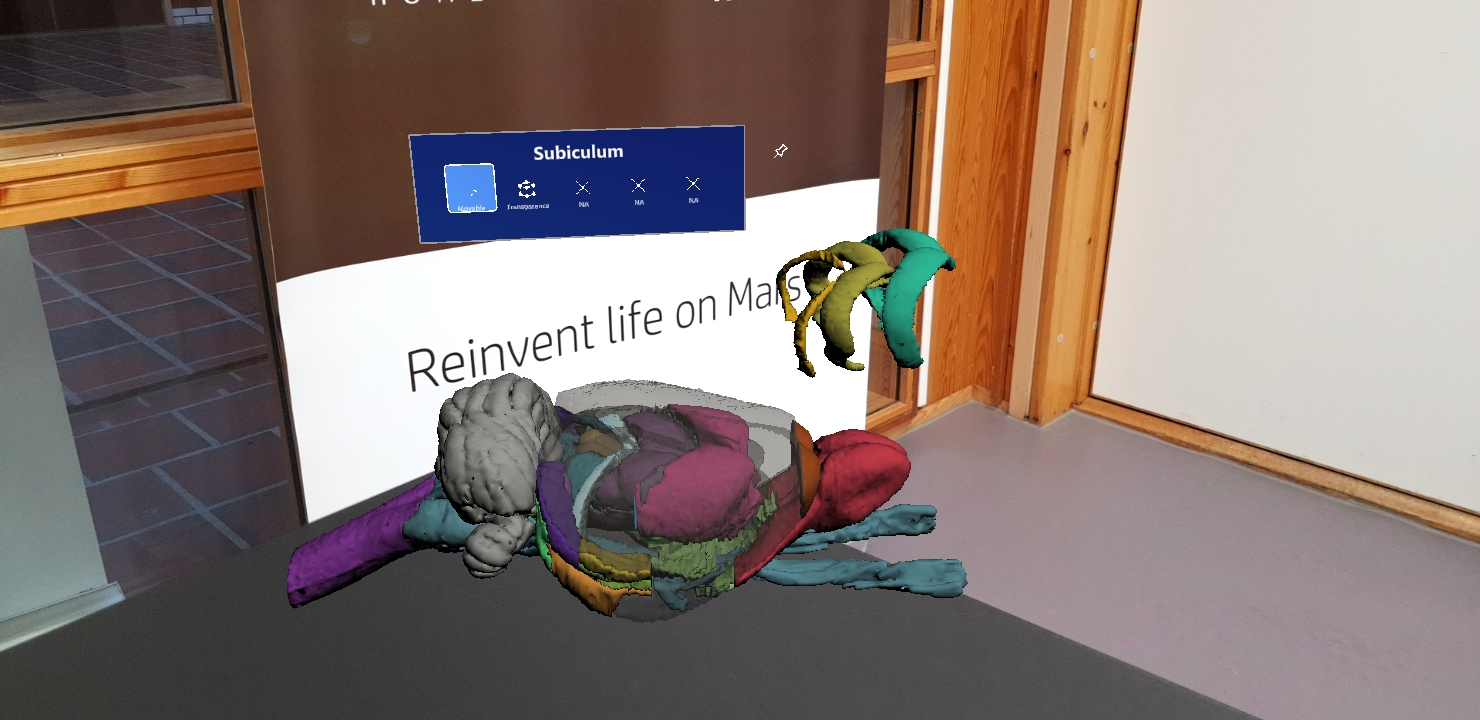
\includegraphics[width=0.5\textwidth]{fig/nevrolens/android_partsout.jpg}
%     \caption{Nevrolens v0.1.3 on Android}
% \end{figure}





% \section{Results}

% Because of the COVID-19 pandemic no user testing has been done this semester, in fact no medical students or professionals have tried the application in-person. Thus, it has been difficult to do formal interviews or gather much feedback, especially regarding interaction. This project is the preliminary work for my master thesis next semester and result gathering will naturally be a much more in focus then. And though no user testing has found place, we have arranged live demoes with \nameref{chap:wdp} over Zoom, which have generated useful feedback. 
% In one such demonstration, I wore a HoloLens 2 and use Nevrolens with guidance from a neuroscientist to extract related regions of the brain and was lectured on their role in behavior. 
% The feedback on its use for a single user, was that there should be a global list menu to toggle different features on each brain part, that there should be ability to increase resolution of a single brain part and some way to visualize microscopical data. 

% % Mostly, the feedback has been positive

% % Success in picking out brain parts, and explaining different structures in the brain. 



% % results from this project are limited.